\chapter{Obsah CD a manuál pro spuštění a vyhodnocení experimentů}

Přiložené CD obsahuje zdrojové texty k této diplomové práci, framework ECJ
\footnote{\url{https://cs.gmu.edu/~eclab/projects/ecj/}}\footnote{\url{https://cs.gmu.edu/~eclab/projects/ecj/docs/manual/manual.pdf}},  který obsahuje zdařilou implementaci genetického
programování, zdrojové texty k experimentům a zdrojové texty k programům na vyhodnocení experimemtů. Obsah příloženého CD
je na nejvyšší úrovni organizován následovně:
\begin{verbatim}
.
|-- Code
|-- Text	
\end{verbatim}
, kde složka \texttt{Code} obsahuje všechno potřebné pro spuštění a vyhodnocení experimentů a složka \texttt{Text} obsahuje zdrojové
texty k textu této práce, které je možno přeložit standartním způsobem za použití systému \texttt{Make}.

Framework ECJ je uložen ve složce \texttt{Code/ecj} a jeho součástí jsou i experimenty s návrhem hašovacích funkcí \texttt{Code/ecj/ec/iphashing}. 
Hierarchii experimentů je organizovaná následovně:
\begin{verbatim}
iphashing
|-- func
|-- experiments
|-- problems
    |-- byoctet
        |-- terms
        |-- IPHashing.java
        |-- basicRun.params
    |-- cuckoo
        |-- terms
        |-- Cuckoo.java
        |-- cuckoo.params
    |-- merkledamgard
        |-- terms
        |-- merkledamgard.params
        |-- MerkleDamgard.java
\end{verbatim}
Složka \texttt{func} obsahuje implementaci všech funkčních symbolů, které mohou být použity v jednotlivých experimentech. Složka \texttt{problems}
obsahuje implementaci jednotlivých sad experimentů, \texttt{byoctet} obsahuje implementaci návrhu přímou metodou, \texttt{merkledamgard} implementaci
optimalizace Merkle-Damg\r{a}rdova schématu a \texttt{cuckoo} implementaci návrhu pro kukaččí hašování. Framework ECJ je jen velmi obtížně 
parametrizovatelný, takže každý experiment obsahuje i vlastní sadu terminálních symbolu obsažené ve složkách \texttt{terms}, které se navzájem
téměř neliší. Každý experiment obsahuje také vlastní nastavení pro genetické programování, tato nastavení jsou obsažena v souborech
s příponou \texttt{params}.


\section{Spuštění a vyhodnocení experimentů zaměřených na návrh hašovacích funkcí}
Experimenty obsažené ve složce \texttt{experiments} je nutné spouštět z nadřazené složky \texttt{Code/ecj} a každému experimentu obsaženému
v práci náleží jeden skript ve skriptovacím jazyku \texttt{bash}:
\begin{verbatim}
cd Code/ejc
bash ec/iphashing/experiments/merkleDamgard.sh
\end{verbatim}
Spustí experimenty s návrhem hašovacích funkcí pro Merkle-Damg\r{a}rdovo schéma. Skript spustí 50 nezávislých běhů, jejichž výstupy ukládá do složky, kterou
je možné měnit v hlavičce skriptu. Je nutné počítat s tím, že běh experimentu nějakou dobu trvá. 
Volba datasetů, nad kterými mají algoritmy běžet, je nutné provést přímo ve zdrojových
textech jednotlivých experimentů (\texttt{IPHashing.java}, \texttt{Cuckoo.java} a \texttt{MerkleDamgard.java}), protože framework ECJ neumožňuje
tuto volbu parametrizovat.

Máme-li naše experimenty ukončené, můžeme je začít vyhodnocovat. K tomu souží programy ve složce \texttt{Code/data-scripts}. Jsou zde 
dva programy naimplementované v jazyce Haskell \texttt{avgPopulation} pro výpočet průměrné populace a \texttt{avgBest} pro výhodnocení
nejlepšího dosaženého řešení. Programy je možné přeložit za použití programu \texttt{stack} (standartní metoda překládání balíčků v jazyce
Haskell) následovně:
\begin{verbatim}
cd Code/data-scripts
stack build
\end{verbatim}
\texttt{stack} stáhne správnou verzi kompilátoru GHC, všechny nutné závislost a programy přeloží. Ty jsou uloženy v pracovní složce \texttt{.stack-work},
ale jejich spouštění je usnadněno programem \texttt{stack}. \texttt{stack exec avgPopulation} nebo \texttt{stack exec avgBest}. Oba dva programy berou
jako první povinný argument složku s experimenty. Program \texttt{avgPopulation} bere jako druhý povinný argument počet kvantilů a jako třetí argument
cílový kvantil pro výpis. Tímto způsobem je možné vypsat medián, první nebo třetí kvartil a podobně. Příkazy
\begin{verbatim}
avgPopulation <složka s experimenty> 4 2
avgPopulation <složka s experimenty> 4 1
avgPopulation <složka s experimenty> 4 3
\end{verbatim}
je možné získat průměrný běh pro medián, první nebo třetí kvartil. Příkazem \texttt{avgBest} je možné spustit vyhodnocení nehořsího a nejlepšího řešení
mezi danými experimenty, prvního a třetího kvartilu a medián. Tyto výstupy jsou vhodné pro konstrukci krabicových diagramů. 

\section{Spuštění experimentů zaměřených na rychlost hašovacích funkcí}
Experimenty s rychlostí hašovacích funkcí jsou obsažené ve složce \texttt{Code/hashes-speed-experiments}. Experimenty jsou napsány v jazyce C++ 
ve standardu 11. Je nutné mít nainstalován kompatibilní kompilátor \texttt{gcc}. Přeložení experimentu se provádí standartně systémem \texttt{Make} v
dané složce:
\begin{verbatim}
cd Code/hashes-speed-experiments
make
./speedtest
\end{verbatim}

\section{Spuštění ostatních experimentů}
Součástí balíku jsou ještě experimenty s některými konvečními hašovacími funkcemi pro vyhodnocení jejich práce nad zadanými datasety. Experimenty
jsou obsaženy ve složce \texttt{Code/generic-hashes-experiments}. Experimenty jsou realizovány v jazyce Haskell a je možné je přeložit stejným způsobem
jako v předešlém případě. 
\begin{verbatim}
cd Code/generic-hashes-experiments
stack build
\end{verbatim}
Překlad vytvoří spustitelné soubory \texttt{murmurhash3-experiments}, \texttt{farmhash-experiments}, \texttt{cityhash-experiments} a také jedné evolučné
navržené hašovací funkce \texttt{ip-hashing-experiments} pro ověření správnosti evolučního algoritmu. Je možné je spustit programem \texttt{stack} následovně:
\begin{verbatim}
cd Code/generic-hashes-experiments
stack exec murmurhash3-experiments
stack exec farmhash-experiments
stack exec cityhash-experiments
stack exec ip-hashing-experiments
\end{verbatim}

\chapter{Článek a plakát na konferenci Excel@FIT 2016}
Předběžné výsledky této práce byly publikovány na konference Excel@FIT 2016. Příspěvek byl vybrán
odbornou komisí k ústní prezentaci. Práce získala ocenění odborného panelu za nekonvenční přístup k návrhu hašovacích
funkcí pomocí evolučního algoritmu a ocenění odbornou veřejností za excelentní práci a její prezentaci během přehlídky.

\newpage
\begin{figure}[!ht]
	\centering 
	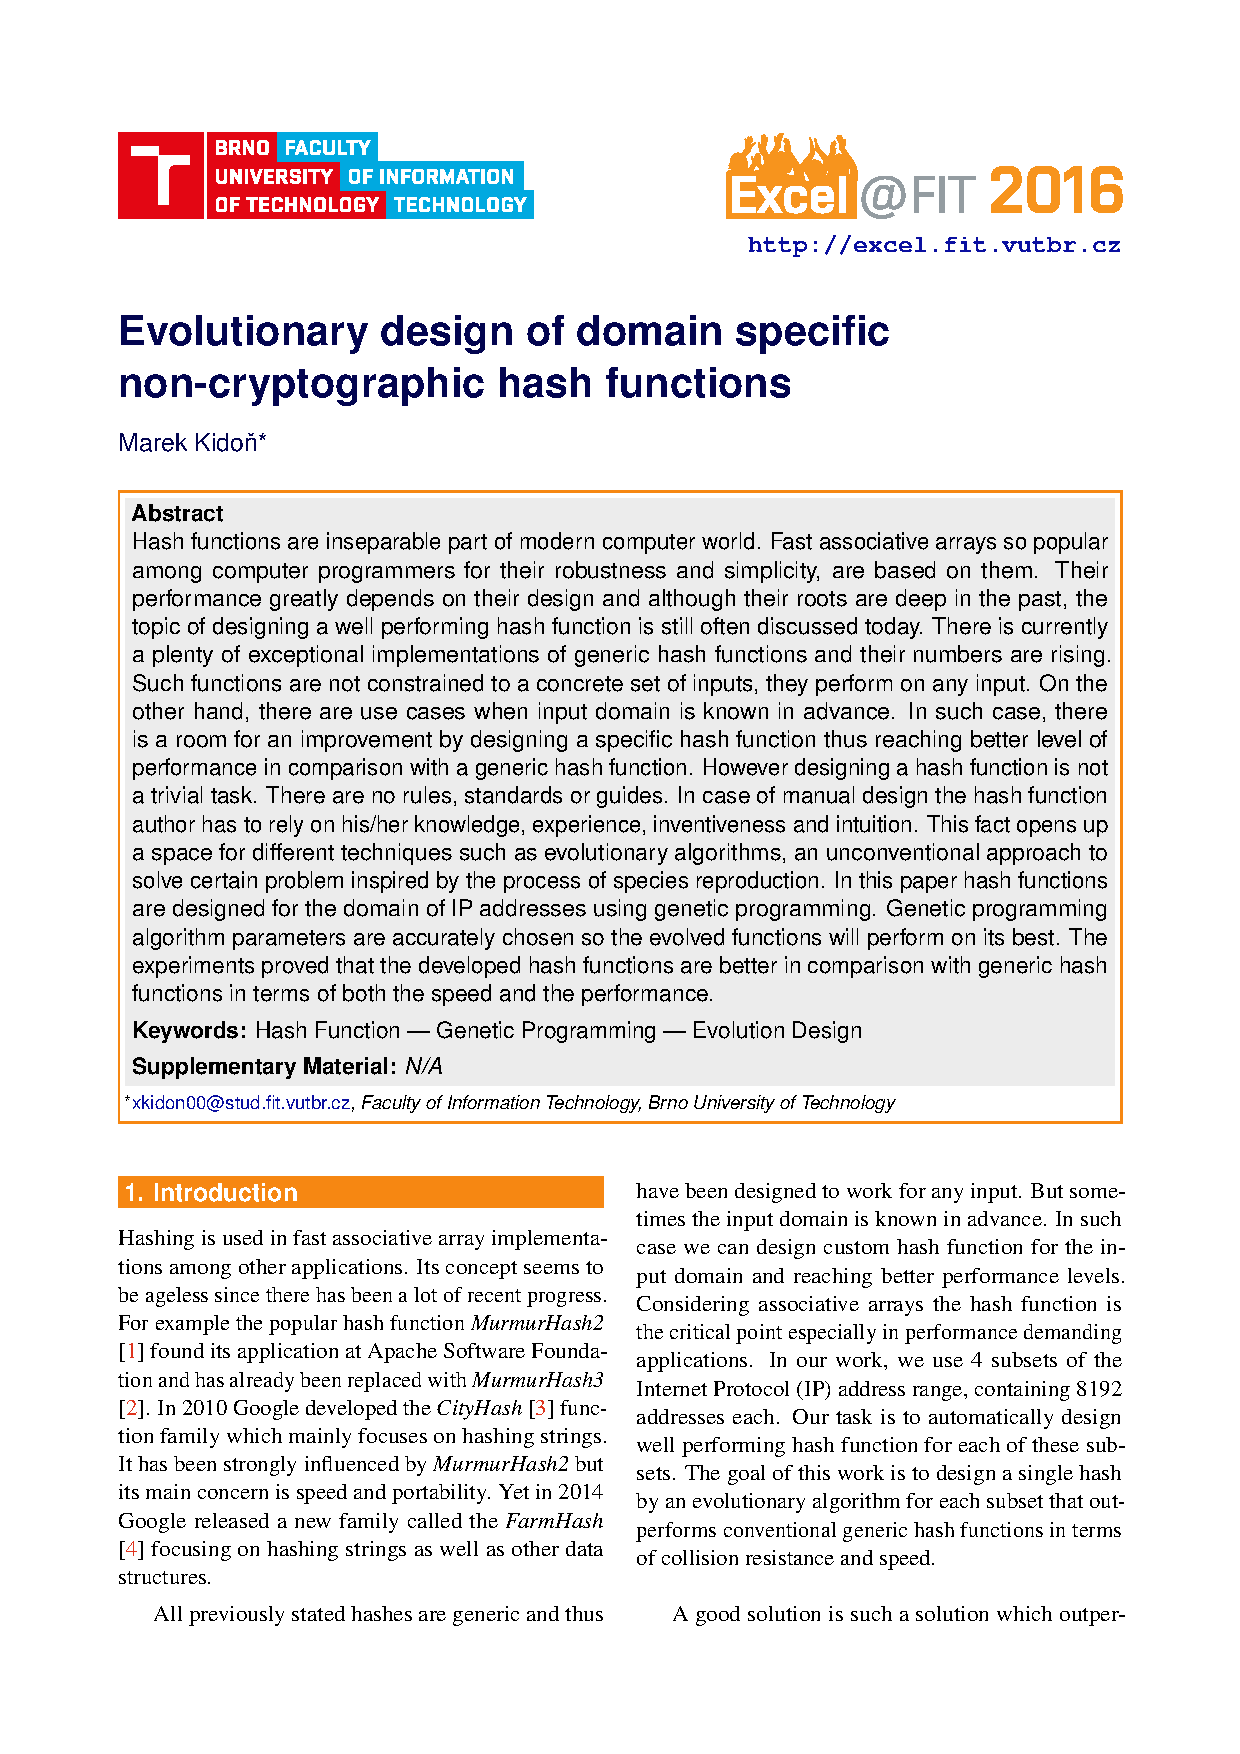
\includepdf[pages=1]{includes/ExcelFITPaper.pdf}
\end{figure}
\newpage
\begin{figure}[!ht]
	\centering 
	\includepdf[pages=2]{includes/ExcelFITPaper.pdf}
\end{figure}
\newpage
\begin{figure}[!ht]
	\centering 
	\includepdf[pages=3]{includes/ExcelFITPaper.pdf}
\end{figure}
\newpage
\begin{figure}[!ht]
	\centering 
	\includepdf[pages=4]{includes/ExcelFITPaper.pdf}
\end{figure}
\newpage
\begin{figure}[!ht]
	\centering 
	\includepdf[pages=5]{includes/ExcelFITPaper.pdf}
\end{figure}
\newpage
\begin{figure}[!ht]
	\centering 
	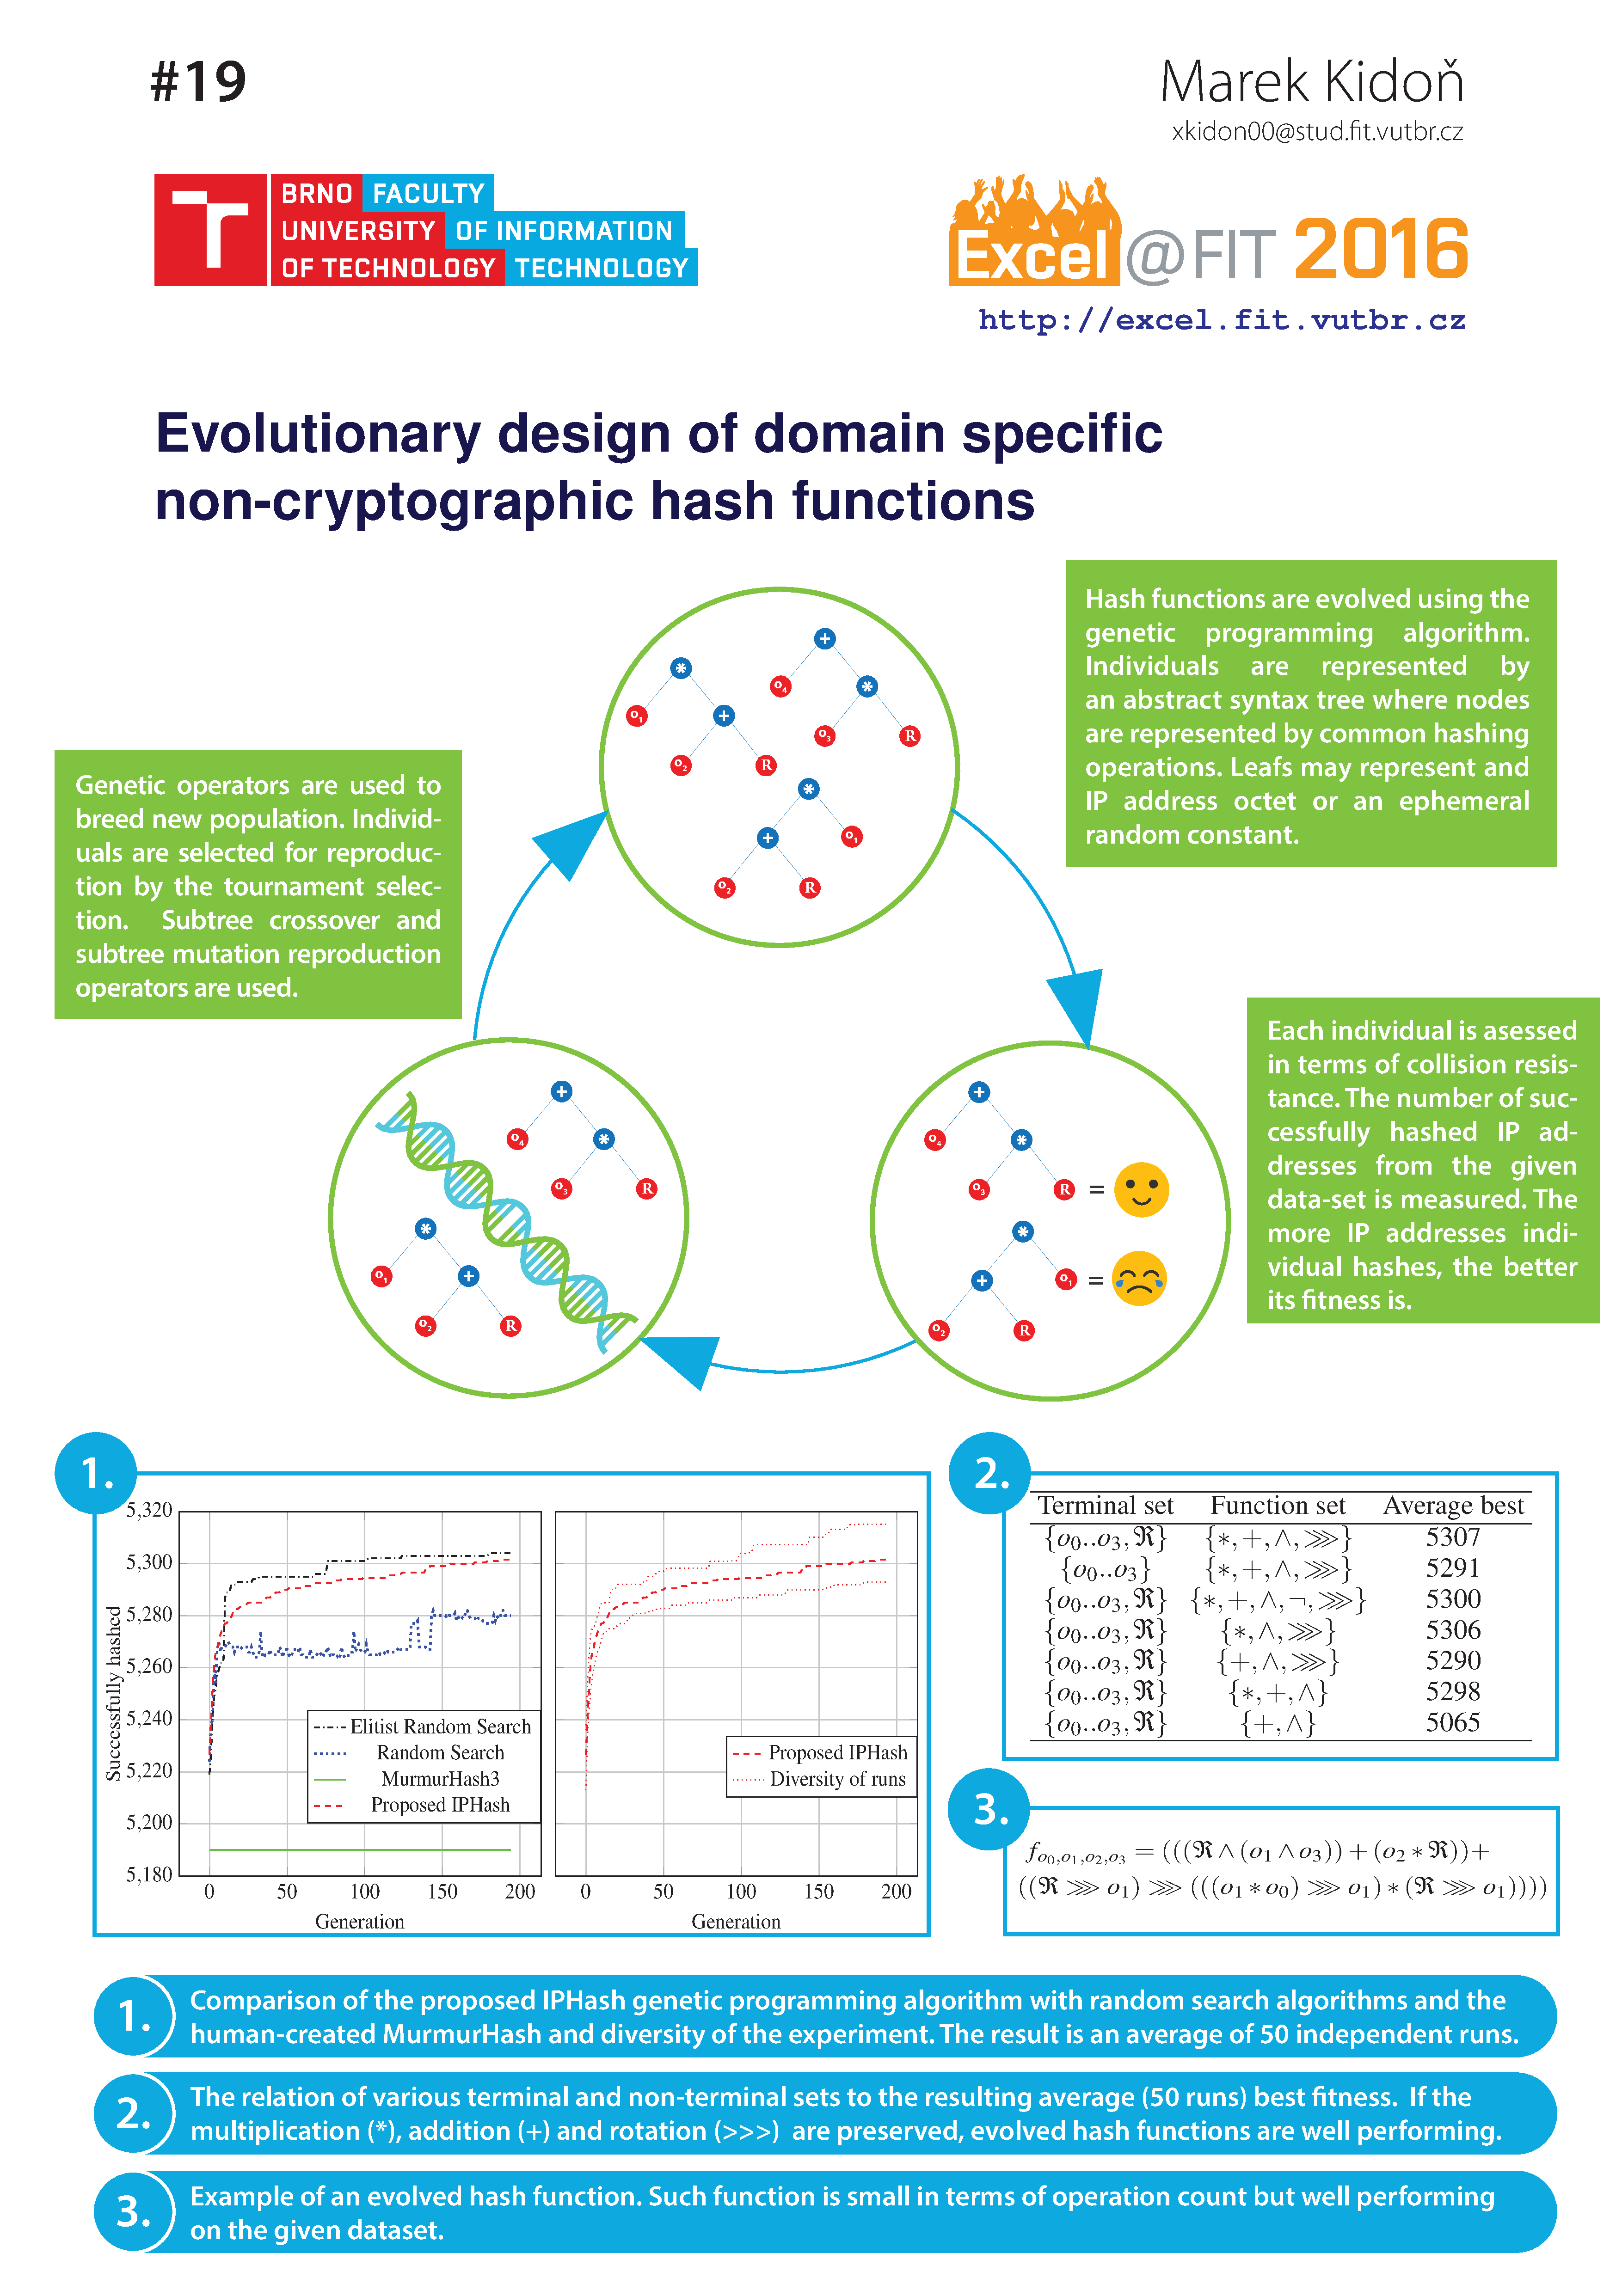
\includepdf{includes/ExcelFITPoster.pdf}
\end{figure}

